\documentclass[11pt]{article}

\usepackage[margin=0.6in]{geometry}
\usepackage[T1]{fontenc}
\usepackage[utf8]{inputenc}
\usepackage{lmodern}
\usepackage{array}
\usepackage{booktabs}
\usepackage{longtable}
\usepackage{tabularx}
\usepackage{caption}
\usepackage{float}
\usepackage{hyperref}
\usepackage{parskip}
\usepackage{ragged2e}
\usepackage{setspace}
\usepackage{enumitem}
\usepackage{needspace}
\usepackage[table]{xcolor}
\usepackage{tikz}
\usetikzlibrary{arrows.meta,fit,positioning}
\usepackage[natbibapa]{apacite}

\definecolor{PrimaryRed}{HTML}{8B1E1E}
\definecolor{DeepNavy}{HTML}{15324A}
\definecolor{SoftBlue}{HTML}{DDEEFF}
\definecolor{SoftGreen}{HTML}{E4F1E8}
\definecolor{SoftGold}{HTML}{F8EDC7}
\definecolor{SoftRose}{HTML}{F5E2E7}
\definecolor{SoftGray}{HTML}{F4F4F4}
\definecolor{MidTeal}{HTML}{287D7A}

\hypersetup{
  colorlinks=true,
  linkcolor=DeepNavy,
  urlcolor=DeepNavy,
  citecolor=DeepNavy,
  pdftitle={Words That Have Evidence: A Dignity-Centered Positive Classroom Support Plan},
  pdfauthor={Piter Zacari Garcia Bautista},
  pdfsubject={EDE 448 Module 2 Positive Classroom Support Plan},
  pdfkeywords={positive classroom support, positive self-talk, productive failure, Identity Beads, Puzzle Plan, EQUITAS}
}
\setlength{\parindent}{0pt}
\setstretch{1.08}
\setlist[itemize]{leftmargin=0.23in,itemsep=0.025in,topsep=0.05in}
\setlist[enumerate]{leftmargin=0.28in,itemsep=0.025in,topsep=0.05in}
\captionsetup{font=small,labelfont=bf,labelsep=period}
\bibliographystyle{apacite}

\newcommand{\reviewsection}[1]{%
  \Needspace{4\baselineskip}
  \vspace{0.08in}\noindent{\normalsize\bfseries\color{PrimaryRed}#1}
  \par\vspace{0.025in}
}

\newcommand{\plansubhead}[1]{%
  \Needspace{3\baselineskip}
  \vspace{0.04in}\noindent{\small\bfseries\color{DeepNavy}#1}
  \par\vspace{0.015in}
}

\newcommand{\tableheaderthree}[3]{%
  \rowcolor{PrimaryRed}
  \color{white}\bfseries #1 &
  \color{white}\bfseries #2 &
  \color{white}\bfseries #3 \\
}

\begin{document}

\hypersetup{pageanchor=false}
\begin{titlepage}
\newgeometry{margin=0.7in}
\thispagestyle{empty}

\begin{center}
{\large University of Rochester\\}
{\normalsize Warner School of Education\\[0.15in]}

{\color{PrimaryRed}\rule{\textwidth}{1.4pt}}\\[0.12in]
{\Huge\bfseries Words That Have Evidence}\\[0.15in]
{\huge A Dignity-Centered Positive\\[0.06in]
Classroom Support Plan}\\[0.12in]
{\Large Positive Self-Talk, Identity Recognition,\\[0.04in]
and Access-to-Agency}\\[0.14in]
{\large EDE 448 --- Module 2 Assignment}\\[0.10in]

\vfill

{\color{PrimaryRed}\rule{0.78\textwidth}{0.7pt}}\\[0.18in]

\colorbox{SoftBlue}{%
\parbox{0.88\textwidth}{%
\centering\small\vspace{0.02in}
\textbf{Positive Does Not Mean Pretending Everything Is Fine}\\[0.04in]
Credible self-talk begins with real evidence, honors what a learner feels and communicates, and leads to a support, choice, or next action that actually exists.
}%
}
\end{center}

\vfill

\begin{center}
\renewcommand{\arraystretch}{1.18}
\setlength{\tabcolsep}{4pt}
\begin{tabular}{>{\bfseries\RaggedLeft}p{1.85in} p{5.0in}}
Student & Piter Zacari Garcia Bautista \\
Assignment & Positive Classroom Support Plan \\
Course & EDE 448 --- Communication and Positive Behavioral Supports for Students with Autism and Other Complex Needs \\
Future Setting & Inclusive, technology-rich upper-elementary or middle school classroom \\
Applied Experience & EDU486 Invisible Invaders camp and Identity Beads \\
Interpretive Framework & Puzzle Plan, with EQUITAS at its heart \\
Due Date & July 31, 2026, 11:59 PM EDT \\
\end{tabular}
\end{center}

\vfill

\begin{center}
\begin{minipage}{0.92\textwidth}
\centering\itshape
The goal is to help students recognize evidence, communicate what they need, and author a fuller story about what they can do.\\
{\color{PrimaryRed}\rule{4.2in}{0.8pt}}
\end{minipage}
\end{center}

\vfill

\begin{center}
\begin{minipage}{0.95\textwidth}
\small
This plan is guided by my Puzzle Plan, an interdisciplinary framework that connects lived experience, education, data, and research so that no single label, behavior, observation, or score is mistaken for the whole learner. EQUITAS is the equity-centered heart of the Puzzle Plan. It asks whose knowledge is included, what context is missing, how power and bias shape interpretation, and whether a decision expands access, dignity, agency, and belonging. Through those connected commitments, positive self-talk becomes one part of accessible classroom design rather than a demand that students privately overcome public barriers.
\end{minipage}
\end{center}

\restoregeometry
\end{titlepage}
\hypersetup{pageanchor=true}
\pagenumbering{arabic}

\reviewsection{What Makes a Classroom Support Truly Positive}

My future classroom will include students who differ in communication, sensory processing, movement, executive functioning, language, culture, disability, chronic illness, prior technology access, energy, and comfort with group work. I will not measure a positive classroom by how consistently students look calm, attentive, cheerful, or socially typical. I will measure it by whether students can understand what is happening, communicate in dependable ways, use meaningful supports, enter rigorous learning, protect boundaries, repair harm, and remain recognized as full members of the community.

This distinction matters for positive self-talk. A student who says, ``I cannot do this,'' may be expressing fear, overload, pain, missing background knowledge, an inaccessible first step, a history of being underestimated, or a correct judgment that the present conditions do not work. Replacing that sentence immediately with ``I am amazing'' may sound positive while ignoring the evidence. A stronger response begins with curiosity: What part feels impossible? What happened before? What tool, model, person, communication route, or pause would change the situation? What has the learner already done that can support a believable next statement?

Positive behavior support is strongest when goals are socially meaningful and outcomes include quality of life, participation, collaboration, and sustainable change \citep{dunlap2012pbs}. First-hand accounts also warn that interventions can produce masking, shame, trauma, and weakened boundaries when adult-defined normality becomes the hidden goal \citep{gardner2017firsthand}. Positive self-talk must therefore increase a learner's choices and access. It cannot become forced optimism, emotional surveillance, or another way to make distress less visible to adults.

This paper builds on my submitted Module 2 assignment, \textit{From Compliance to Communication: Prevent--Teach--Reinforce Planning Through Access, Agency, and Richer Evidence} \citep{garciabautista2026ptr}. That earlier paper used one teaching-placement transition to examine behavior as evidence, separate observation from inference, and show how participation changed when an adult changed the access condition. I do not repeat its case-based PTR analysis here. Instead, this plan carries its central commitment into whole-class design and extends it through positive self-talk, Identity Beads, accessible routines, and an explicit examination of how adults and institutions assign meaning to failure.

\reviewsection{Positive Self-Talk Works Best When the Words Are Believable}

Research gives me a more precise starting point than ``think positive.'' In a randomized field experiment with students in Grades 4--6, effort-focused self-talk supported mathematics performance for children with negative competence beliefs, whereas general ability-focused self-talk did not produce the same benefit \citep{thomaes2020effort}. That study does not prove that one phrase works for every learner or every task. It does suggest that believable language about effort and action may be more useful than broad claims about being inherently good at something.

Work on reading intervention similarly treats recognizing negative thoughts and using positive self-talk as teachable self-regulation practices, while cautioning that instruction must not overload working memory or displace explicit academic teaching \citep{dahlleonard2023selftalk}. In my classroom, the language must therefore be brief, concrete, relevant to the task, and connected to an available action. Examples include:

\begin{itemize}
  \item ``I do not know the first step \textit{yet}; I can ask to see one.''
  \item ``My body is giving me information; I can pause, adjust, and return.''
  \item ``This result is evidence. I can test one change.''
  \item ``I can use speech, typing, drawing, pointing, AAC, or a partner to show what I know.''
  \item ``One difficult moment is not the whole story. I can name what I contributed.''
\end{itemize}

No learner will be required to say these words aloud, disclose an internal thought, or adopt a teacher-written affirmation. Self-talk may remain internal or be represented through text, symbols, AAC, gesture, a private card, a digital prompt, or partner-supported communication. Jorgensen's call to construct communicative competence means that the classroom must make those routes available throughout the day, including during stress, refusal, transition, and repair \citep{jorgensen2018competence}.

\reviewsection{Who Decides Whether Failure Is Negative?}

Schools and society often teach a hidden equation: an unsuccessful result is negative, and a person who produces it is less capable, less intelligent, or less worthy. Adults teach that equation through grades that erase revision, public comparison, praise reserved for speed and first-try correctness, and language such as ``you failed'' rather than ``this attempt did not yet meet the goal.'' A child can then inherit an adult judgment as self-talk: ``I failed, therefore I am a failure.''

I want to teach a more accurate distinction. Language that threatens safety, encourages self-harm, dehumanizes, or attacks a person's identity is harmful and requires protection and repair. An error, uncertainty, frustration, disappointment, or an attempt that did not work is different. It can be painful or uncomfortable without being evidence of a bad learner. We can name real harm without defining the harmed student, the student's emotion, or an ordinary learning experience as negative.

Learning research supports this reframing, with important conditions. A review of error-based learning found that errors can strengthen learning when they are followed by corrective feedback and analysis of the reasoning that produced them; error tolerance can also support active exploration \citep{metcalfe2017errors}. A meta-analysis of problem-solving-before-instruction designs found benefits for conceptual knowledge and transfer when Productive Failure principles were implemented with fidelity, while also identifying differences by age and learning goal \citep{sinha2021productivefailure}. Failure does not teach automatically. It becomes usable learning when students have low-stakes opportunities, accessible feedback, instruction, reflection, support, and another attempt.

Mastery is not a record of unbroken success. It is a history of attempts, feedback, revision, changed strategies, and increasingly informed judgment. Nobody becomes an expert because every first attempt worked; expertise grows in part from learning what did not work, why it did not work, and what to change next.

This changes the language I will model and invite students to adapt:

\begin{itemize}
  \item ``I failed at this attempt, and now I know what did not work. I am better informed than I was yesterday.''
  \item ``I do not know this yet, but I learned \underline{\hspace{0.75in}}. I can use that evidence for the next part.''
  \item ``I will learn this the way I learned \underline{\hspace{0.75in}}: with time, practice, feedback, support, and more than one route.''
  \item ``The strategy failed; I did not become a failure.''
\end{itemize}

\begin{figure}[H]
\centering
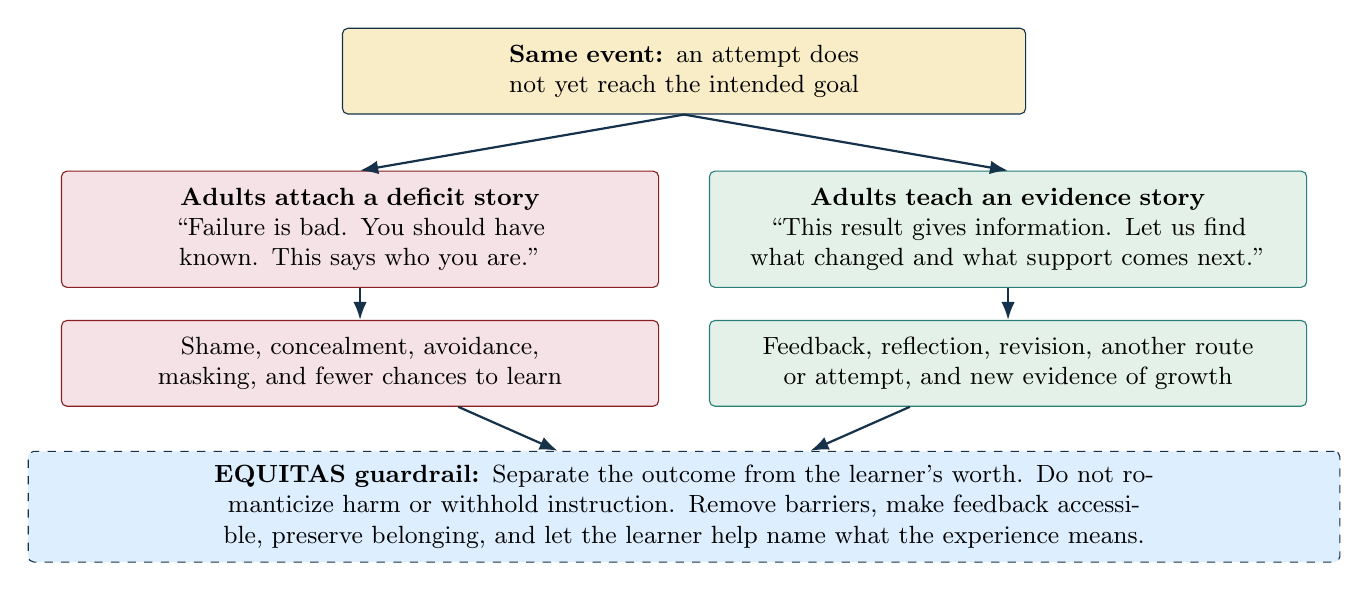
\begin{tikzpicture}[
  meaningflow/.style={-{Latex[length=2.3mm]}, line width=0.8pt, draw=DeepNavy},
  eventbox/.style={draw=DeepNavy, rounded corners=2pt, fill=SoftGold,
    text width=3.25in, align=center, inner sep=6pt, font=\small},
  judgmentbox/.style={draw=PrimaryRed, rounded corners=2pt, fill=SoftRose,
    text width=2.82in, align=center, inner sep=6pt, font=\small},
  evidencebox/.style={draw=MidTeal, rounded corners=2pt, fill=SoftGreen,
    text width=2.82in, align=center, inner sep=6pt, font=\small},
  guardrail/.style={draw=DeepNavy, dashed, rounded corners=2pt, fill=SoftBlue,
    text width=6.42in, align=center, inner sep=5pt, font=\small}
]
\node[eventbox] (attempt) {\textbf{Same event:} an attempt does not yet reach the intended goal};
\node[judgmentbox, below=0.28in of attempt, xshift=-1.62in] (deficit) {\textbf{Adults attach a deficit story}\\``Failure is bad. You should have known. This says who you are.''};
\node[evidencebox, below=0.28in of attempt, xshift=1.62in] (learning) {\textbf{Adults teach an evidence story}\\``This result gives information. Let us find what changed and what support comes next.''};
\node[judgmentbox, below=0.16in of deficit] (narrow) {Shame, concealment, avoidance, masking, and fewer chances to learn};
\node[evidencebox, below=0.16in of learning] (expand) {Feedback, reflection, revision, another route or attempt, and new evidence of growth};
\node[guardrail, below=0.22in of narrow, xshift=1.62in] (guardrail) {\textbf{EQUITAS guardrail:} Separate the outcome from the learner's worth. Do not romanticize harm or withhold instruction. Remove barriers, make feedback accessible, preserve belonging, and let the learner help name what the experience means.};
\draw[meaningflow] (attempt.south) -- (deficit.north);
\draw[meaningflow] (attempt.south) -- (learning.north);
\draw[meaningflow] (deficit) -- (narrow);
\draw[meaningflow] (learning) -- (expand);
\draw[meaningflow] (narrow) -- (guardrail);
\draw[meaningflow] (expand) -- (guardrail);
\end{tikzpicture}
\caption{The unsuccessful attempt is the same; adult language, social meaning, and available support shape what the learner is positioned to carry forward. The left path is not caused by failure itself.}
\label{fig:failure-meaning}
\end{figure}

\reviewsection{What Identity Beads Taught Me About Evidence and Recognition}

The "Invisible Invaders" camp made this idea concrete. On July 28, youth sieved saved sand, documented litter, examined tire-wear residue, participated in a synthetic-tissue filtration model, and discussed environmental questions. At the end of the day, the Identity Beads activity invited them to recognize forms of participation they had demonstrated, including designing, investigating, inventing, advocating, motivating, storytelling, bravery, care for others, and a self-described contribution \citep{campteam2026day3,campteam2026identity}. The beads did not need to say, ``I am good at science because an adult says so.'' They could support a more grounded sentence: ``I investigated because I compared what changed,'' or ``I advocated because I connected evidence to environmental action.'' The physical bead made the reflection visible, but the evidence gave the bead meaning. Our documentation also maintained an important boundary: a bead recognized a contribution from that day; it did not rank youth, diagnose a trait, or permanently define anyone's identity.

That design aligns with Mercier and Carlone's distinction between Identi-Beads for self-recognition and Identi-Badges for recognition by others \citep{mercier2021identibeads}. Their account emphasizes multiple, fluid modes of STEM engagement. It warns that recognition systems can become meaningless tokens or hierarchies if categories are treated as fixed or if adults notice only the most visible performances. Recognition should broaden what counts as competence to include quiet contribution, care, advocacy, revision, and collaboration. Our camp's final recognition reinforced the same principle: identity grows through doing meaningful work, seeing oneself in that work, and being recognized by people who matter \citep{campteam2026showcase}. I cannot claim from our records that one activity caused a lasting identity change for any participant. I can say that the activity created a structured opportunity for evidence-based self-recognition without requiring youth to compete for one definition of a scientist.

\reviewsection{The Evidence-Based Self-Talk Cycle}

The cycle below turns positive self-talk into a process of reflection and access. A statement is not the starting point. The learner first notices what is happening, examines evidence and context, selects believable language in an accessible mode, uses a real support or next action, and reflects on what changed. The cycle can begin again with new evidence.

\begin{figure}[H]
\centering
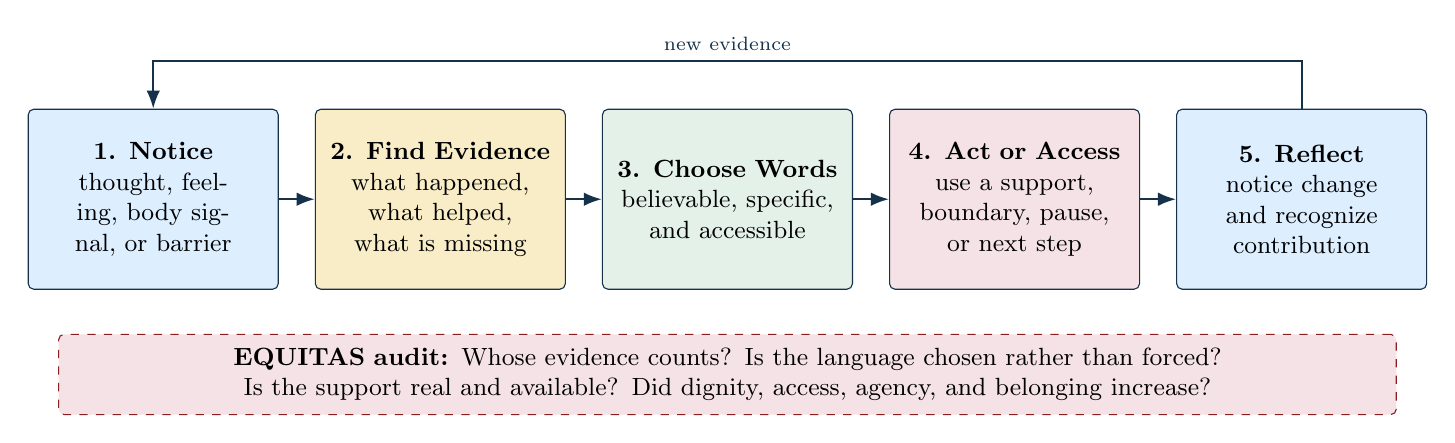
\begin{tikzpicture}[
  node distance=0.18in,
  cyclestep/.style={draw=DeepNavy, rounded corners=2pt, minimum width=1.25in,
    text width=1.12in, minimum height=0.90in, align=center, font=\small},
  flow/.style={-{Latex[length=2.3mm]}, line width=0.8pt, draw=DeepNavy},
  audit/.style={draw=PrimaryRed, dashed, rounded corners=2pt, fill=SoftRose,
    text width=6.55in, align=center, inner sep=5pt, font=\small}
]
\node[cyclestep, fill=SoftBlue] (notice) {\textbf{1. Notice}\\thought, feeling, body signal, or barrier};
\node[cyclestep, fill=SoftGold, right=of notice] (evidence) {\textbf{2. Find Evidence}\\what happened, what helped, what is missing};
\node[cyclestep, fill=SoftGreen, right=of evidence] (words) {\textbf{3. Choose Words}\\believable, specific, and accessible};
\node[cyclestep, fill=SoftRose, right=of words] (act) {\textbf{4. Act or Access}\\use a support, boundary, pause, or next step};
\node[cyclestep, fill=SoftBlue, right=of act] (reflect) {\textbf{5. Reflect}\\notice change and recognize contribution};
\draw[flow] (notice) -- (evidence);
\draw[flow] (evidence) -- (words);
\draw[flow] (words) -- (act);
\draw[flow] (act) -- (reflect);
\coordinate (returnright) at ([yshift=0.24in]reflect.north);
\coordinate (returnleft) at ([yshift=0.24in]notice.north);
\draw[flow] (reflect.north) -- (returnright) -- node[above, font=\scriptsize, text=DeepNavy]{new evidence} (returnleft) -- (notice.north);
\node[audit, below=0.22in of words] (audit) {\textbf{EQUITAS audit:} Whose evidence counts? Is the language chosen rather than forced? Is the support real and available? Did dignity, access, agency, and belonging increase?};
\end{tikzpicture}
\caption{An original five-step cycle for evidence-based positive self-talk. The EQUITAS audit remains active across every step.}
\label{fig:self-talk-cycle}
\end{figure}

\reviewsection{A Self-Talk and Access Menu}

The menu is not a script students must memorize. It is a set of examples for co-creating language that remains honest and actionable.

\small
\begin{longtable}{>{\RaggedRight\arraybackslash}p{1.47in} >{\RaggedRight\arraybackslash}p{2.55in} >{\RaggedRight\arraybackslash}p{2.55in}}
\tableheaderthree{Moment or Message}{Evidence-Linked Language}{Support or Next Action}
\endfirsthead
\tableheaderthree{Moment or Message}{Evidence-Linked Language}{Support or Next Action}
\endhead
``I cannot do this.'' &
``I do not know the first step yet. I can ask to see one.'' &
Completed example, visual model, one direction, chosen partner, or teacher demonstration. \\
\rowcolor{SoftGray}
``Everyone is faster.'' &
``Speed is not the learning goal. I can show my thinking through another route.'' &
Remove unnecessary timing; offer typing, drawing, AAC, oral explanation, photograph, or extended processing time. \\
Sensory load, pain, or fatigue &
``My body is giving me information. I can adjust, pause, or use a lower-energy route.'' &
Quieter location, sensory tool, movement, seating change, familiar device, break, or visible re-entry point. \\
\rowcolor{SoftGray}
An unsuccessful attempt or unexpected result &
``This attempt did not reach the goal, and it taught me what did not work. I can use that evidence to revise.'' &
Specific feedback, error analysis, comparison example, debugging guide, material reset, chosen support, or another low-stakes trial. \\
Peer conflict or boundary &
``I can say stop, name what happened, and ask for help repairing it.'' &
Speech, writing, symbols, AAC, private report, mediation, recovery time, and a clear re-entry plan. \\
\rowcolor{SoftGray}
Identity threat &
``One moment is not the whole picture. I can name evidence of how I contributed.'' &
Private evidence card, Identity Bead or digital symbol, portfolio artifact, peer recognition with permission, or teacher documentation. \\
\end{longtable}
\normalsize

\reviewsection{Using Identity Beads Without Turning Identity Into a Reward System}

I would adapt the camp activity as a weekly or project-end reflection, not as a token economy. Students could choose a bead, digital symbol, color, word, or no artifact at all. The process would be:

\begin{enumerate}
  \item Review broad, co-created contribution categories and invite student-defined additions.
  \item Select evidence from the day or project: an observation, question, design move, revision, act of care, boundary, explanation, or contribution.
  \item Choose an identity word or symbol that fits that evidence today.
  \item Complete an optional stem such as, ``I was an investigator when I\ldots'' or ``I want to recognize that I\ldots'' through any accessible mode.
  \item Choose whether the reflection stays private, enters a portfolio, or is shared.
  \item Offer peer or adult recognition only when it cites observable evidence and respects the learner's preference.
\end{enumerate}

There will be no bead totals, leaderboards, required categories, public comparison, or assumption that one color permanently defines a learner. A student can choose several identities, create a new one, decline the activity, or change the meaning over time. Adults will actively notice contributions that schools often overlook, including listening, translating, regulating, questioning an assumption, supporting access, using AAC, protecting an evidence boundary, or returning after a difficult moment.

\reviewsection{Routine-by-Routine Implementation}

The Edutopia classroom-management session emphasizes structure, predictability, relationships, transitions, and instructional clarity \citep{edutopiaClassroom}. Those ideas inform the routines below, but they also require adult reflection. When I do not understand a student's response, I need to say, ``I do not understand this yet; I can gather evidence and ask the student,'' rather than defend my first interpretation because I am supposed to have every answer.

\small
\begin{longtable}{>{\RaggedRight\arraybackslash}p{1.02in} >{\RaggedRight\arraybackslash}p{1.93in} >{\RaggedRight\arraybackslash}p{2.15in} >{\RaggedRight\arraybackslash}p{1.46in}}
\rowcolor{PrimaryRed}
\color{white}\bfseries Routine &
\color{white}\bfseries Classroom Design and Access &
\color{white}\bfseries Self-Talk or Communication Route &
\color{white}\bfseries Evidence to Review \\
\endfirsthead
\rowcolor{PrimaryRed}
\color{white}\bfseries Routine &
\color{white}\bfseries Classroom Design and Access &
\color{white}\bfseries Self-Talk or Communication Route &
\color{white}\bfseries Evidence to Review \\
\endhead
Arrival &
Visible agenda, calm entry task, greeting options, consistent materials, private check-in. &
``What do I need to begin?'' through speech, gesture, symbol, device, or private response. &
Entry route, support selected, transition to first task. \\
\rowcolor{SoftGray}
Mini-lesson &
Purpose, short model, one direction, visual example, processing time. &
``I can identify one thing I understand and one thing I need shown.'' &
First step begun, question asked, route used. \\
Hands-on or digital work &
Stable materials, role choices, debugging guide, sensory and movement options, meaningful extension. &
``I noticed\ldots,'' ``I tested\ldots,'' ``My first attempt taught me\ldots,'' ``I can try\ldots,'' or ``I need\ldots'' &
Questions, revisions, contribution, tool access, peer dynamics. \\
\rowcolor{SoftGray}
Transition, break, and return &
Warning, first/next visual, overlap, familiar support, nonpunitive reset area, named re-entry step. &
``Not yet,'' ``more time,'' ``keep this with me,'' ``break,'' or ``I am ready to return.'' &
Latency, distress, communication, recovery, successful entry or return. \\
Closure and recognition &
Protected time, prompt shown early, multiple response modes, optional Identity Bead or evidence card. &
``Today I contributed by\ldots'' or a student-created alternative; private, shared, or passed. &
Whose work was recognized, whose mode was accessible, what students want next. \\
\end{longtable}
\normalsize

Zacarian and Silverstone's classroom-community planning reminds me that support begins before a problem: with names, language, accommodations, strengths, sensory and physical access, family communication, and important relationships \citep{zacarian2015community}. Family and student knowledge will be invited rather than extracted. No learner should have to disclose a diagnosis, trauma, poverty, culture, pain, or family hardship to earn an accessible route.

\reviewsection{How I Will Know Whether the Plan Is Working}

I will not count the number of positive statements students produce and call that success. My review data will include:

\begin{itemize}
  \item whether learners can choose or create believable language in an accessible mode;
  \item whether learners can separate an outcome from their worth and identify what an unsuccessful attempt taught them without being forced to describe harm as positive;
  \item whether requests for help, pause, refusal, another tool, or re-entry receive dependable responses;
  \item whether students can identify evidence of contribution without adult prompting;
  \item whose contributions receive peer and adult recognition and whose remain overlooked;
  \item participation, recovery, communication, academic access, safety, and belonging;
  \item student and family judgments about whether the strategy is useful, acceptable, and respectful;
  \item adult implementation fidelity, including whether promised supports were actually available; and
  \item whether changes in visible behavior are accompanied by increased trust and agency.
\end{itemize}

If students repeat the desired words while losing communication, regulation, trust, or access, the plan has failed. If a phrase does not help, the team should examine the language, the task, the support, the hypothesis, and adult implementation before deciding that the learner is resistant. Positive behavior support requires continued evidence-based revision, not loyalty to an intervention because adults designed it \citep{dunlap2012pbs}.

\reviewsection{Puzzle Plan and EQUITAS: Changing the Story and the System}

This plan is personal because I know how institutional descriptions can become internal language. As a Latino Dominican, bilingual, neurodivergent, and chronically ill learner and educator, I have experienced access barriers being interpreted as a character flaw: fatigue as lack of commitment, difficulty with an inaccessible process as irresponsibility, or communication difference as evidence that the thinking matters less. Positive self-talk cannot ask a student to correct privately a story that an inequitable system keeps producing publicly.

The Puzzle Plan keeps the relevant pieces connected: lived experience, student work, communication, family knowledge, classroom design, data, research, culture, disability, tools, peers, and adult response. EQUITAS, as its heart, asks whose knowledge becomes credible evidence, whose competence is recognized, whose language or communication mode is treated as legitimate, and who is expected to sound confident before receiving support.

EQUITAS also asks who is allowed to fail safely. Some students receive time, coaching, revision, and the assumption that they will improve; others have a first error treated as proof that they do not belong. Fairness requires changing that social meaning. I will not pretend that every harmful event was ``for the best,'' but I will refuse the equation that a painful or unsuccessful experience makes the learner negative. We can interrupt harm, preserve the truth of what happened, and still help students use experience as part of the foundation from which they build their own world.

Applied here, fairness does not mean giving every student the same affirmation. It means ensuring that students have real conditions from which believable, self-authored language can grow. One learner may use an internal phrase, another may point to an evidence card, another may keep a bead, another may reject the activity, and another may need the environment changed before any reframing is appropriate. Inclusion means that none of those routes lowers the learner's right to rigor, dignity, or belonging.

\reviewsection{Conclusion}

My positive classroom support plan begins before self-talk. It begins with a visible learning route, multiple ways to communicate and participate, sensory and regulation access, meaningful choices, family and student knowledge, and adults willing to revise the environment. Within those conditions, positive self-talk can become a useful bridge from uncertainty to action.

I will teach failure explicitly as an event and a source of evidence, not as an identity. A learner may say, ``I failed at this attempt, and I know more than I knew before,'' because the classroom provides feedback, support, revision, and another chance. The point is not to make failure sound pleasant. The point is to stop society's judgment from turning one result into a verdict about a person's intelligence, character, or future.

The Identity Beads experience clarified what that bridge can look like. Youth did real work first. Reflection then helped make contribution visible, and recognition expanded the language available for identity. The bead was not the evidence, and the adult did not own the meaning. The strongest message was not ``Be positive.'' It was ``Look at what you did, decide what it means to you, and choose what you want to carry forward.''

That is the classroom culture I want to build: one in which students can name barriers without being defined by them, recognize strengths without pretending difficulty is gone, communicate boundaries without losing belonging, and use evidence to author identities larger than any diagnosis, behavior, score, or adult interpretation.

\small
\bibliography{references}

\end{document}
